\chapter{Конструкторская часть}

На основе формализованных требований к базе данных и выбора её типа может быть выполнено её проектирование.
В данном разделе будут спроектированы сущности базы данных, её ролевая модель а также архитектура погодного приложения.

\section{Проектирование сущностей базы данных}

На этапе анализа определены сущности, которые будут храниться в базе данных.
Необходимо определить тип данных, которым представляется каждый их атрибут, а также атрибуты для идентификации и связи с другими сущностями.
Один из атрибутов каждой сущности -- её идентификатор.
Он представляет собой целое число.
Далее рассмотрена каждая сущность в отдельности.

\subsection*{Погода}
Погода связана с городом, который является отдельной сущностью.
Тогда она должна хранить его идентификатор как внешний ключ, чтобы в базе данных была возможность найти погоду по городу.
Также погода привязана ко времени, которое удобно сделать её атрибутом.
А само время может быть как датой, если рассматривается погода на день, так и часом, если погода почасовая.
Следовательно, сущность погоды должна содержать дату и номер часа, который равен $0$, если она определена для всего дня и лежать в пределах от$1$ до $24$, если она почасовая.
Остальные параметры погоды хранятся как целые и вещественные числа или как строки.
Дополнительными атрибутами погоды являются описание и иконка.
Они нужны для удобства пользователя погодного приложения.

\subsection*{Город и страна}
Далее рассматривается сущность города.
В разных странах могут быть города с одинаковыми названиями.
Поэтому при поиске города пользователю важно выводить не только его название, но и название соответствующей страны.
Таким образом, нужно хранить в базе данных не только города, но и страны.
Так как если хранить название страны как атрибут города, то одна и та же страна может быть по ошибке названа по-разному.
Также город имеет широту и долготу для определения его географического расположения.
В результате к атрибутам города относятся идентификатор, название, внешний ключ страны, широта и долгота.

\subsection*{Иконка погоды}
Для того, чтобы отображать тип погоды в удобном для пользователя формате, необходимо хранить иконку погоды, которая вместе с другими погодными параметрами загружается с сервера.
Такая иконка имеет фиксированный размер $24\times24$ и может храниться как массив байт.
Длина этого массива равна 576, так как каждый пиклель кодируется $4$-байтовым целым числом.

\subsection*{Аккаунт пользователя}
Для реализации ролевой модели необходимо определить сущность пользователя.
Она содержит его идентификатор, роль, имя и пароль.
Перечисленных атрибутов достаточно для определения ролевой модели.
Также в данной сущности пользователя сохраняется дата регистрации аккаунта.
Она может потребоваться в работе приложения.
Таким образом, таблица пользователей будет содержать всю необходимую информацию.

\subsection*{График пользователя}
Приложение предоставляет возможность построения и хранения графиков изменения погодных параметров.
Тогда следует ввести соответствующую сущность.
Шаг построения графика всегда $1$ день, поэтому хранить его не нужно.
Необходимо хранить начальную и конечную дату, название исследуемого параметра, массив его значений, а также внешние ключи автора и города, для котороых строится график.
К дополнительной информации о графике можно отнести его описание, написанное автором.
Перечисленных параметров достаточно для работы с сущностью графика.

\subsection*{Заметка пользователя}
Пользователи приложения имеют возможность делать заметки с комментариями к своим погодным наблюдениям.
Причём над одной заметкой могут работать несколько пользователей.
То есть связь между заметкой и пользователем -- многие ко многим.
Следовательно, нужна не только сущность заметки, но и сущность, хранящая информацию о связи между заметкой и её редакторами.
Для заметки хранится идентификатор, заголовок, текст, время создания и идентификатор автора, который может управлять доступом к ней.
А запись о связи между пользователем и заметкой хранит $3$ атрибута: идентификаторы редактора и заметки, а также время последнего редактирования соответствующим пользователем.
Таким образом, база данных сможет обеспечить правильное хранение отношения пользователей к их заметкам.

\section{Диаграмма сущность-связь}
На рисунках~\ref{fig:er-barker}--\ref{fig:er-chen} представлены диаграммы сущность-связь для разрабатываемой базы данных в нотациях Баркера и Чена.
Они отображают все сущности и связи между ними.
Каждая отдельная сущность соответствует ровно одной таблице в реляционной базе данных.
\begin{figure}[H]
	\centering
	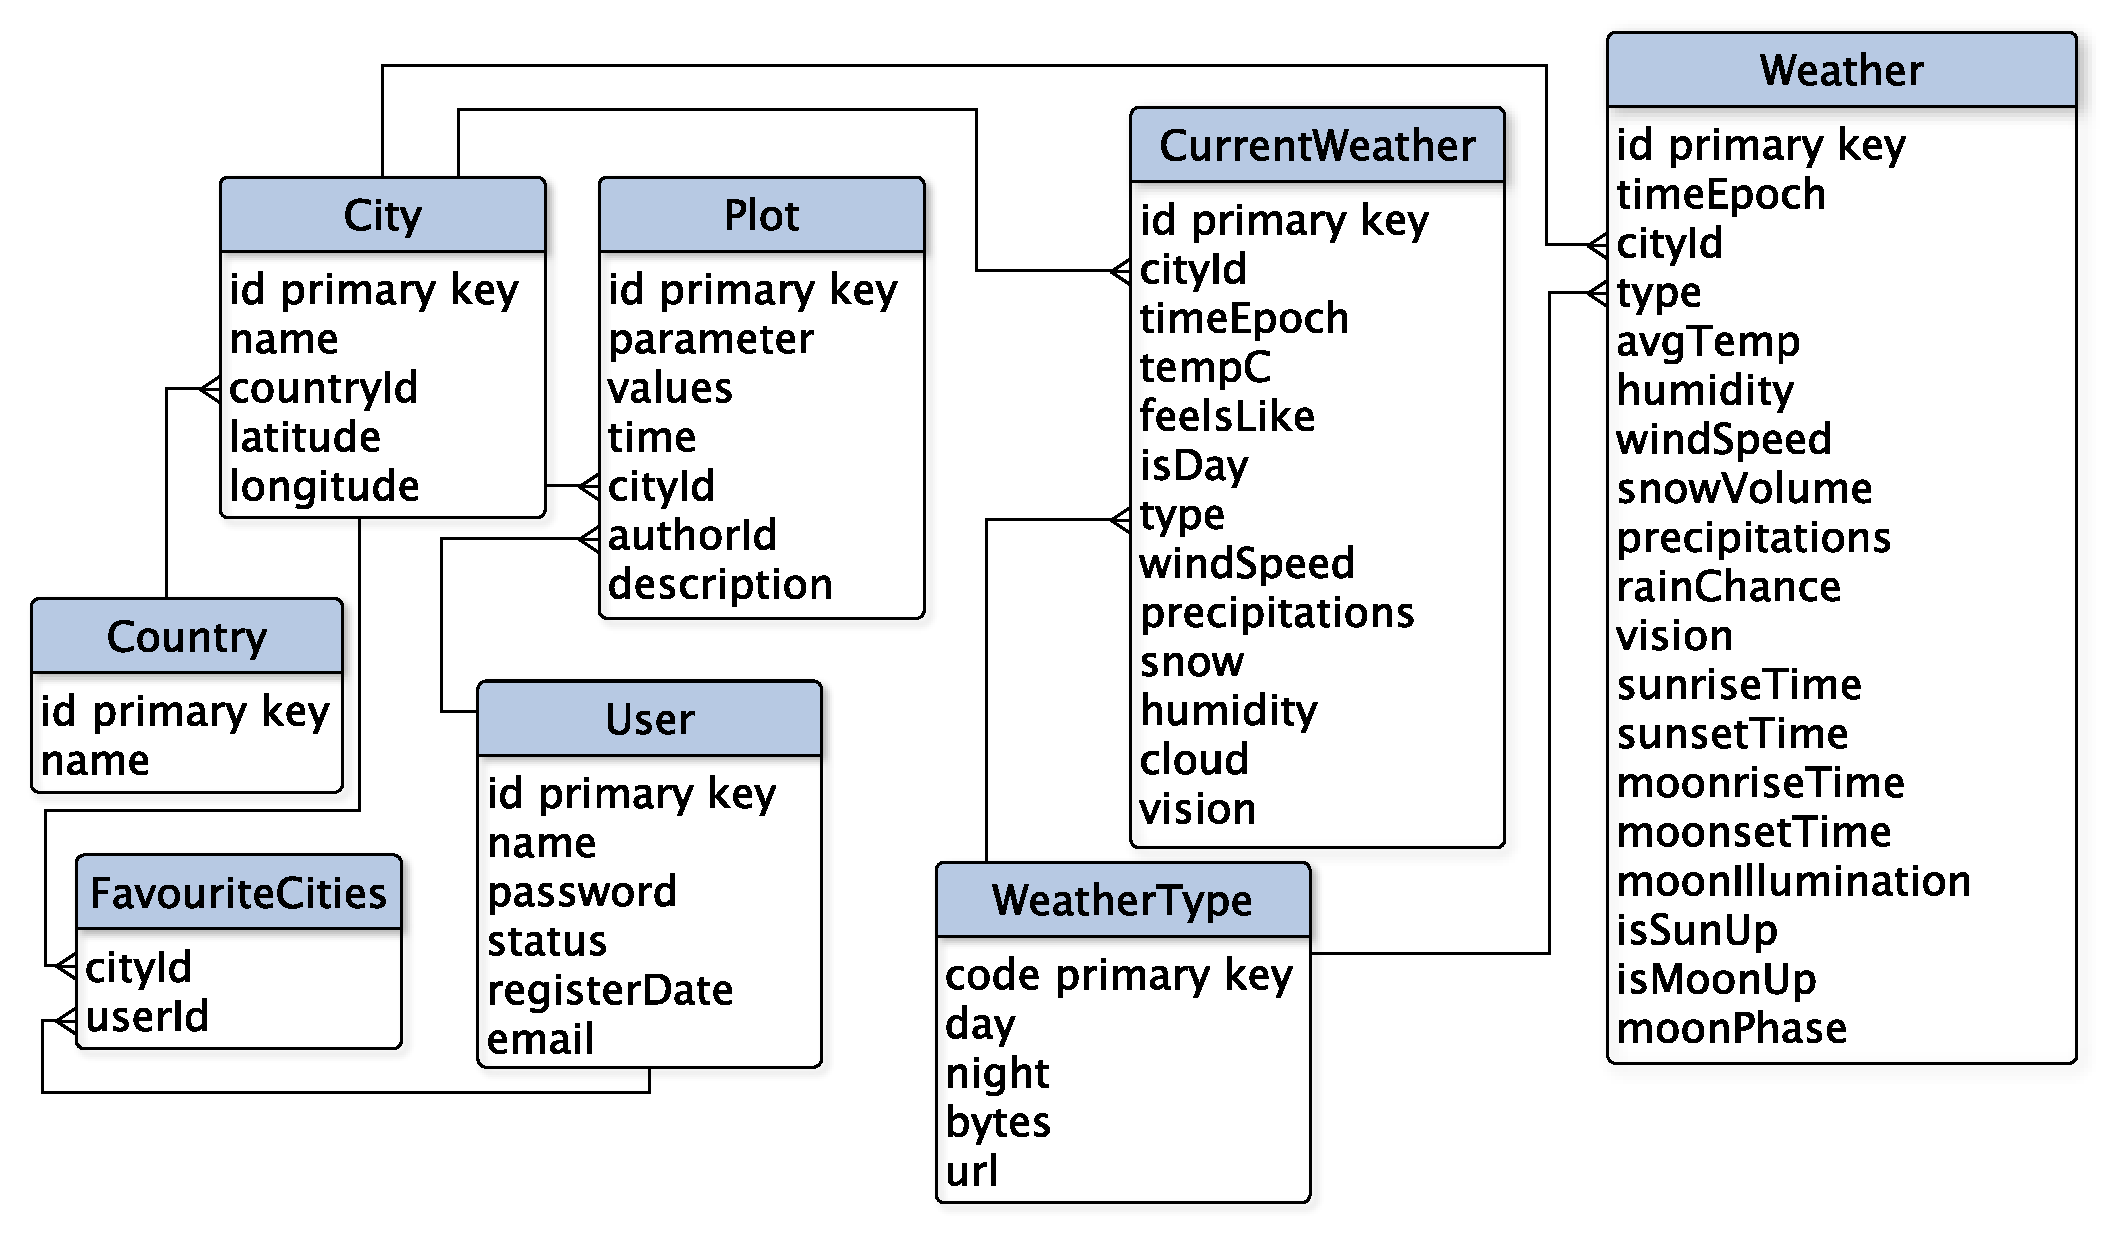
\includegraphics[height=0.45\textheight, width=\textwidth]{tools/img/er-barker.pdf}
	\caption{
        ER-диаграмма разрабатываемой базы данных в нотации Баркера
    }
	\label{fig:er-barker}
\end{figure}

\begin{figure}[H]
	\centering
	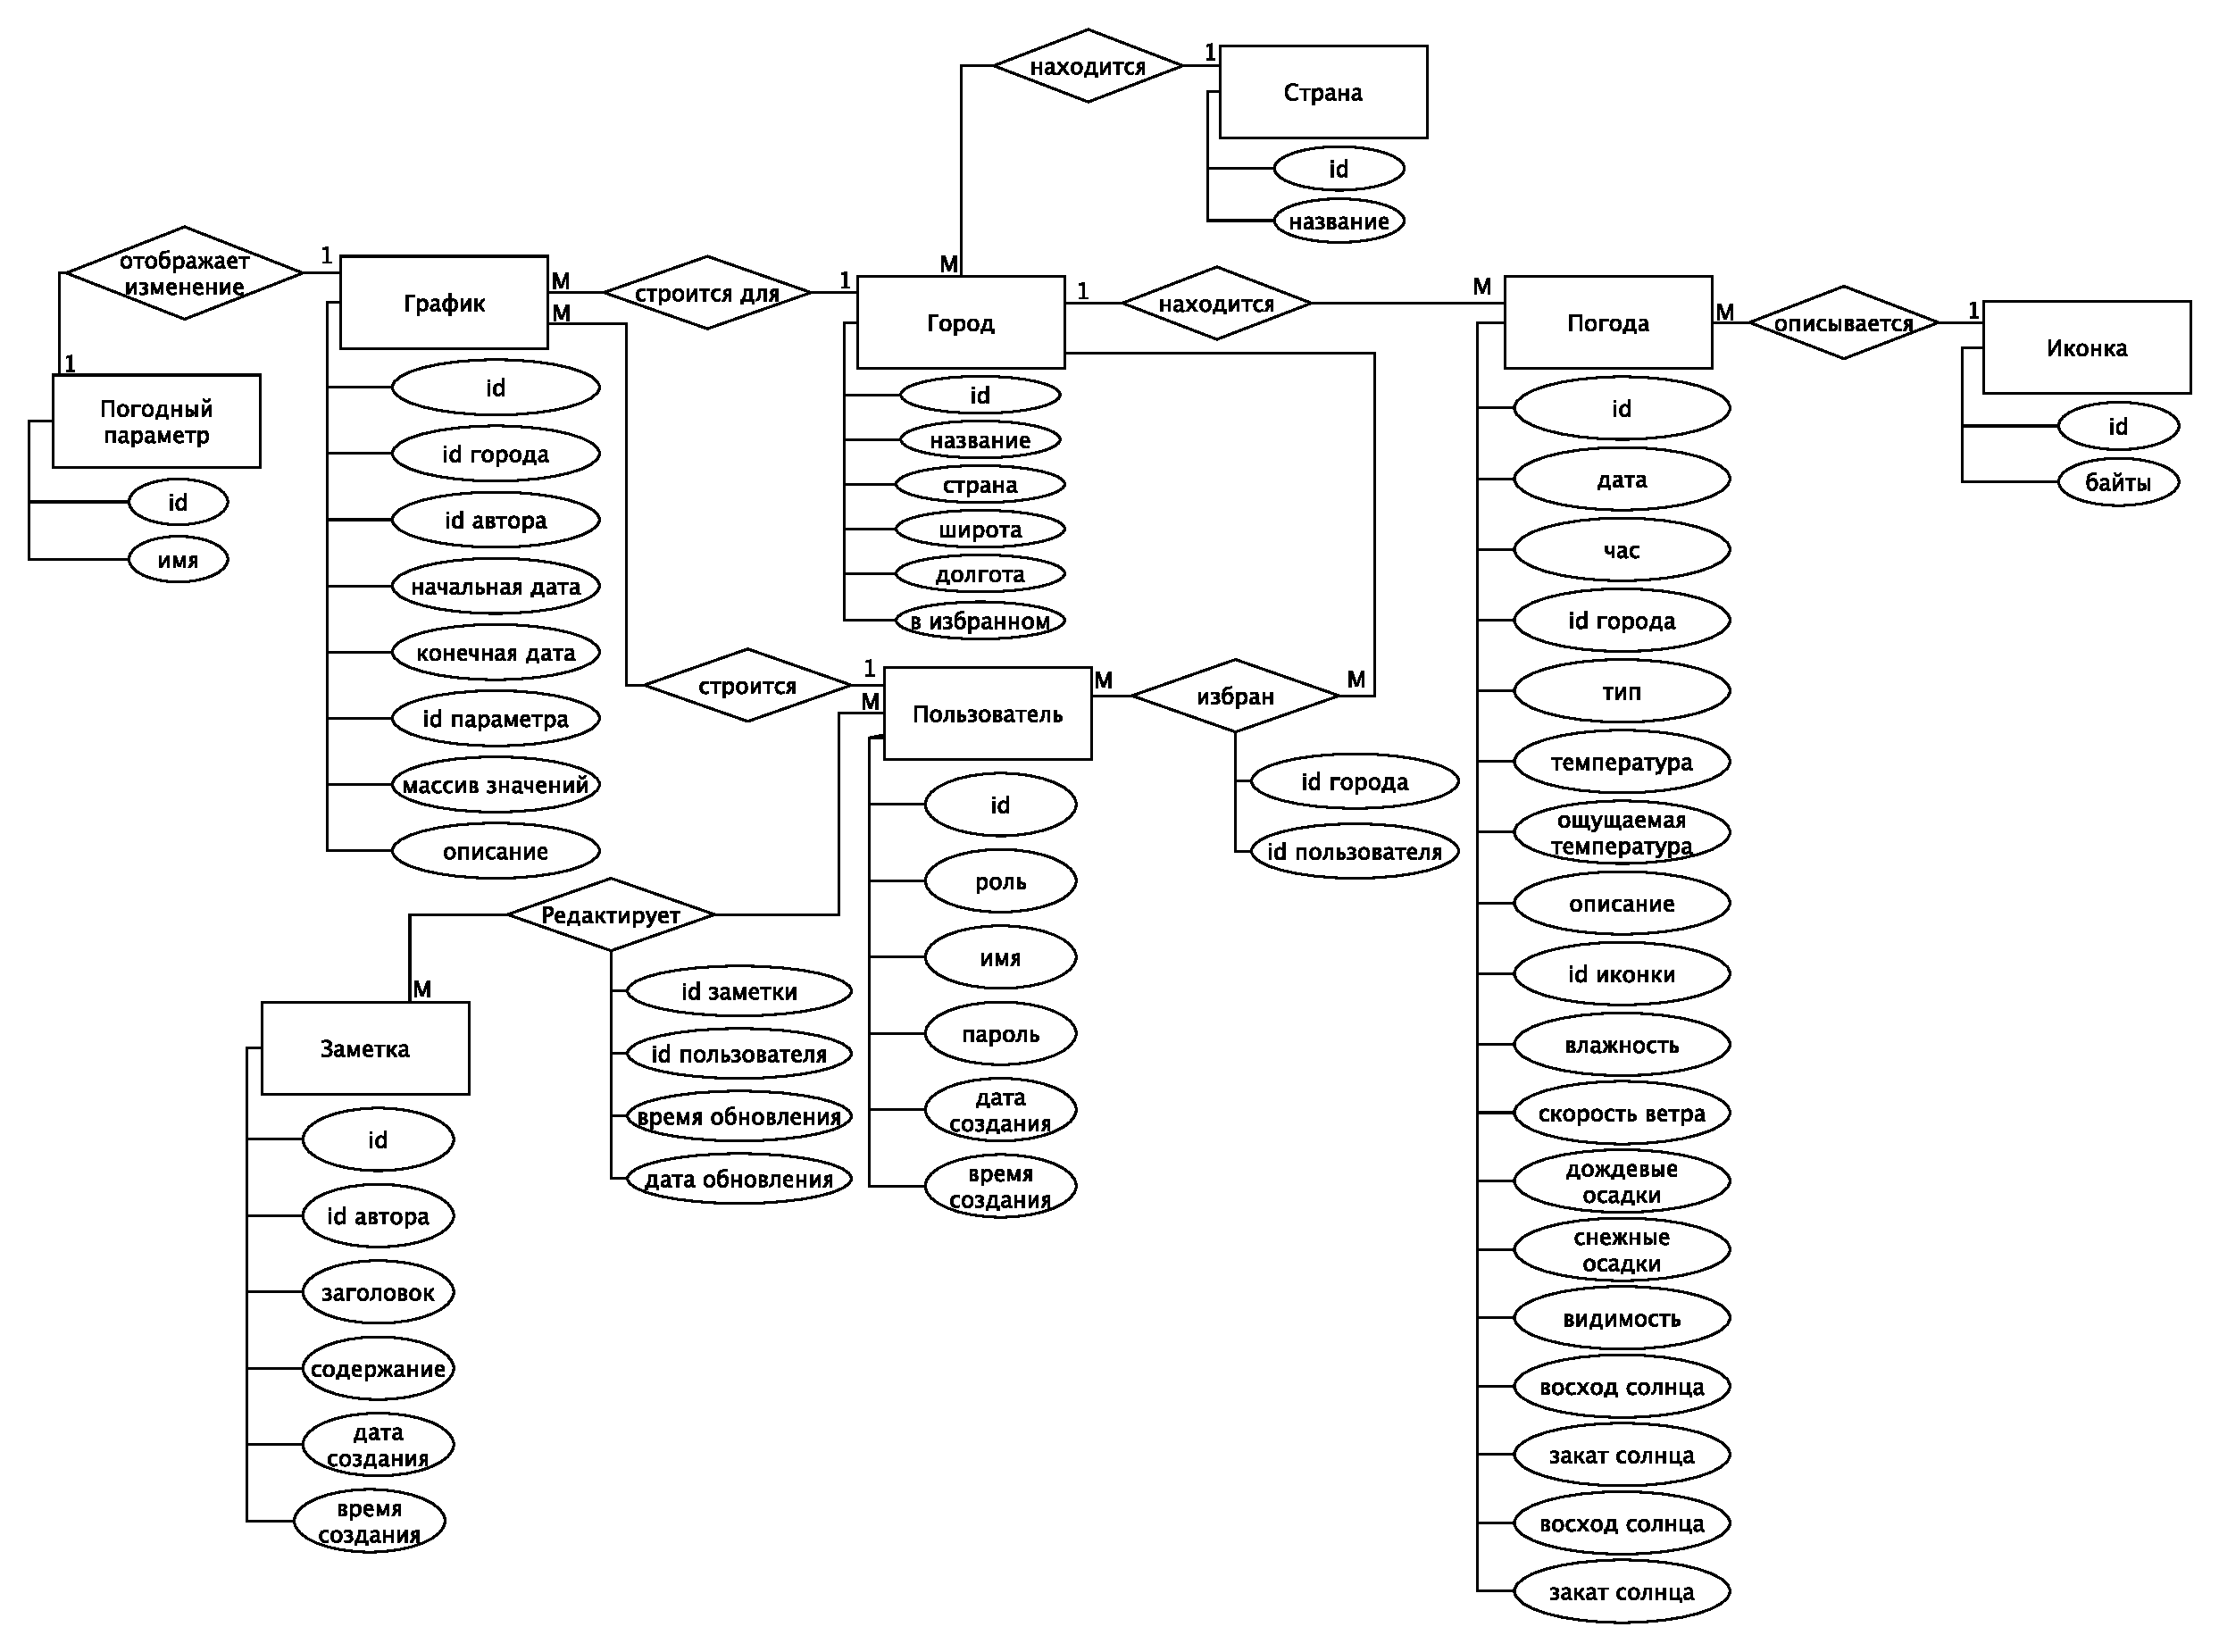
\includegraphics[height=0.6\textheight, width=\textwidth]{tools/img/er-chen.pdf}
	\caption{
        ER-диаграмма разрабатываемой базы данных в нотации Чена
    }
	\label{fig:er-chen}
\end{figure}

\section{Ролевая модель}
Разрабатываемое погодное приложение предполагает ровно $3$ роли пользователей в зависимости от из подписки.
Таким оборазом, пользователи делятся на 3 категории: обычный, продвинутый и премиум пользователь.
Далее представлено описание обязанностей и возможностей каждого пользователя.

\subsection*{Обычный пользователь}
К обычным пользователям относятся те, кто только скачал приложение.
Такому пользователю доступны следующие функции:
\begin{itemize}
    \item получить прогноз погоды не более, чем на 2 дня вперёд;
    \item получить почасовую погоду;
    \item работа со списком избранных городов;
    \item поиск любого города.
\end{itemize}
У обычного пользователя меньше возможностей, чем у пользователя любой другой роли.

\subsection*{Продвинутый пользователь}
Продвинутые пользователи имеют все возможности обычных, плюс следующие:
\begin{itemize}
    \item получить прогноз погоды на месяц вперёд;
    \item получить список дней, когда прогнозируется погода, соответствующая определённым параметрам.
\end{itemize}
К пользователям данной роли относятся те, кто оформил соответствующую подписку.

\subsection*{Премиум-пользователь}
Премиум-пользователи имеют все возможности обычных, плюс следующие:
\begin{itemize}
    \item получить историю погоды;
    \item построить график изменения погодных параметров.
\end{itemize}
К данной роли относятся пользователи, оформившие соответствующую подписку.

\section{Проектирование приложения}
Техническое задание предполагает демонстрацию работы базы данных.
Для этого необходимо написать погодное приложение, использующее её возможности.
Далее перечислены требования к погодному приложению:
\begin{itemize}
    \item
        предоставление возможности использовать любую функцию базы данных;
    \item
        возможность загружать данные о погоде из интернета и сохранять их в базе данных;
    \item иметь графический пользовательский интерфейс.
\end{itemize}

Для реализации приложения была выбрана <<луковичная чистая архитектура>>~[9], а также архитектурный паттерн <<Model-View-Intent>> (MVI).
Таким образом, приложение будет легко поддерживаемым.

\section*{Выводы из конструкторской части}
В данном разделе были спроектированы сущности базы данных и способ их хранения и разработана ролевая модель.
Также спроектирована архитектура приложения, использующего базу данных.
Таким образом, получена достаточная информация для реализации базы данных.